\documentclass[11pt,reqno,a4paper]{amsart}

% set margins
\usepackage[margin=1in]{geometry}


\title{Branched optimal transport}
\date{August 2024}

% Packages
\usepackage{amsmath}
\usepackage{tikz-cd}
\usepackage{amsfonts}
\usepackage{amsthm}
\usepackage{amssymb}
\usepackage{graphicx}

\usepackage{hyperref}\hypersetup{colorlinks=true, citecolor=blue}

\usepackage{biblatex}
\usepackage{textcomp}
\usepackage{mathtools}
\usepackage{stmaryrd}
\addbibresource{bib.bib}

\newenvironment{itemizeb}
{\begin{itemize}
     \itemsep=2pt}{
\end{itemize}}


\numberwithin{equation}{section}

\newtheoremstyle{mytheorem}
{}% measure of space to leave above the theorem. E.g.: 3pt
{}% measure of space to leave below the theorem. E.g.: 3pt
{\it}% name of font to use in the body of the theorem
{\parindent}% measure of space to indent
{\bf}% name of head font
{.}% punctuation between head and body
{ }% space after theorem head; " " = normal interword space
{\thmnumber{#2.~}\thmname{#1}\thmnote{~\rm#3}}% Manually specify head

\newtheoremstyle{myremark}
{}% measure of space to leave above the theorem. E.g.: 3pt
{}% measure of space to leave below the theorem. E.g.: 3ptontinuo dentro e fuori dall'infermeria, poi Barzagli e i due mesi di stop per l'infortunio alla spalla, infine a
{\rm}% name of font to use in the body of the theorem
{\parindent}% measure of space to indent
{\bf}% name of head font
{.}% punctuation between head and body
{ }% space after theorem head; " " = normal interword space
{\thmnumber{#2.~}\thmname{#1}\thmnote{~\rm#3}}% Manually specify head

\newtheoremstyle{myparagraph}
{}% measure of space to leave above the theorem. E.g.: 3pt
{}% measure of space to leave below the theorem. E.g.: 3pt
{\rm}% name of font to use in the body of the theorem
{\parindent}% measure of space to indent
{\bf}% name of head font
{.}% punctuation between head and body
{ }% space after theorem head; " " = normal interword space
{\thmnumber{#2.~}\thmname{#1}\thmnote{#3}}% Manually specify head

\theoremstyle{mytheorem}
\newtheorem{maintheorem}{Theorem}
\newtheorem{theorem}[subsection]{Theorem}
\newtheorem{definition}[subsubsection]{Definition}
\newtheorem{lemma}[subsection]{Lemma}
\newtheorem{corollary}[subsection]{Corollary}
\newtheorem{proposition}[subsection]{Proposition}
\newtheorem{question}[subsection]{Question}

\theoremstyle{myremark}
\newtheorem{remark}[subsection]{Remark}
%\newtheorem*{remark*}{Remark}
%\newtheorem{remarks}[subsection]{Remarks}
%\newtheorem*{remarks*}{Remarks}
\newtheorem{problem}[subsection]{Problem}
\theoremstyle{myparagraph}
\newtheorem{parag}[subsection]{}
\newtheorem*{parag*}{}


\renewcommand\qedsymbol{$\boxempty$}


\newcommand{\R}{\mathbb{R}}


\begin{document}
    \author{Antonio De Rosa, Dario Filatrella, Aida Khajavirad}

    \maketitle


    \tableofcontents
    \newpage

    \nocite{*}


    \section{Introduction}


    \section{Notation and preliminaries}

    \subsection{General notation}

    \begin{itemizeb}
        \leftskip 0.8 cm\labelsep=.3 cm
        \item[$f_{\#}\mu$] push-forward of the measure $\mu$ by a map $f$
        \item[$\mathcal{H}^1$] 1-dimensional Hausdorff measure
        \item[$|\Omega|$] Lebesgue measure of a set $\Omega$ when it is a subset of $\R$
        \item[$T(\gamma)$] Stopping time of a path $\gamma$
        \item[$\|x\|$] Euclidean norm of a vector $x$
        \item[$\R_+^N$] Vectors in $\R^N$ where all components are non-negative
    \end{itemizeb}

    \subsection{Optimal transport notation}
    The following notation will be defined more extensively in the next section but it is summarized here:

    \begin{itemizeb}
        \leftskip 0.8 cm\labelsep=.3 cm
        \item[$N$] Dimension of the space
        \item[$X \subseteq \R^N$] Compact set and domain of the measures
        \item[$K$] Space of 1-Lipschitz paths eventually constant on $X$
        \item[$\mu^+, \mu^-$] Two measures of equal mass on $X$
        \item[$\mathbf{P}$] Traffic plan, measure on $K$ that transports $\mu^+$ to $\mu^-$
        \item[$\pi_0, \pi_\infty$] Maps from $K$ to $X$ defined by $\pi_0(\gamma) = \gamma(0)$ and $\pi_\infty(\gamma) = \gamma(T(\gamma))$
        \item[$\mathcal{E}^{\alpha}(P)$] Gilbert energy of a traffic plan $P$
        \item[$E^{\alpha}(P)$] Energy of a traffic plan $P$
        \item[$\chi$] Parameterization of a traffic plan (with Lagrangian formulation)
        \item[$C(\beta, N)$] Maximum number of non-overlapping caps on a sphere of dimension $N$ (\ref{definition:spherical_cap_results})
    \end{itemizeb}

    \subsection{Discrete branched transport notation}
    The following notation is specific to the discrete branched transport problem (DBT) and its mixed integer non-linear programming formulation (MINLP).
    \begin{itemizeb}
        \leftskip 0.8 cm\labelsep=.3 cm
        \item [$P$] Set of terminals $\{p_1, \ldots, p_n\}$
        \item [$S$] Set of Steiner $\{s_1, \ldots\}$ points (indexed as $S = \{|P| + 1, ..., 2|P|-2\}$)
        \item[$E$] Set of all edges
        \item [$E_1$] Set of edges connecting terminals to Steiner points
        \item [$E_2$] Set of edges connecting Steiner points

        \item[$\alpha \in {[0,1]}$] cost parameter
        \item [$M$] set of masses $\{m_1, \ldots, m_n\}$ of the terminals
        \item [$P^+$] set of terminals with positive masses (sinks)
        \item [$P^-$] set of terminals with negative masses (sources)
        \item [$f_{xy}$] flow on the edge connecting $x$ to $y$
        \item [$y_{xy}$] binary variable indicating the presence of an edge between $x$ and $y$
        \item [$deg(\alpha, N, M)$] maximum degree of a vertex in the graph as defined in \ref{lemma:degree_definition}
    \end{itemizeb}

    \newpage


    \section{Optimal transport definitions}

    We start with the most abstract definition of branched transport, which holds for generic measures $\mu^+$ and $\mu^-$.
    The numerical analysis will be restricted to the discretized case where $\mu^+$ is a Dirac delta and $\mu^-$ is a finite sum of Dirac deltas.

    \subsection{Branched transport \cite[Chapter 3]{Bernot}}

    Given $X \subset \mathbb{R}^N$ compact, $K$ space of 1-Lipschitz path which are eventually constant on $X$ and
    two measures of equal mass $\mu^+$ and $\mu^-$ on $X$, a traffic plan is a measure $\mathbf{P}$ on $K$ that transports $\mu^+$ to $\mu^-$.
    Formally, consider the maps $\pi_0, \pi_\infty : K \rightarrow X$ given by $\pi_0(\gamma) = \gamma(0)$ and $\pi_\infty(\gamma) = \gamma(T(\gamma))$, where $T(\gamma)$
    is the stopping time of the path $\gamma$.
    $\mathbf{P}$ is a traffic plan if:
    \[
        \mu^+ = (\pi_0)_{\#}\mathbf{P}, \quad \mu^- = (\pi_\infty)_{\#}\mathbf{P}
    \]

    \subsection{Parameterized Traffic Plans}
    The next paragraph is copied from~\cite{Bernot}:

    According to Skorokhod theorem~\cite[Theorem A.3]{Bernot}, we can parameterize any traffic plan $\mathbf{P}$ by a measurable function
    $\chi : \Omega = [0, |\Omega|] \rightarrow K$, where $\Omega$ is a measure space which we identify with an interval, such that
    $\mathbf{P}= \chi_{\#} \lambda$, where $\lambda$ is the Lebesgue measure on $[0, |\Omega|]$.
    We shall set $\chi(\omega, t) \coloneqq \chi(\omega)(t)$ and consider it as a function of the variable pair
    $(\omega, t)$.

    With this formulation we can define the \textbf{energy} (or cost) of a parameterized traffic plan as:
    \begin{equation}
        E^{\alpha}(\mathbf{P}) = \int_{\mathbb{R}^N} |x|_\mathbf{P}^{\alpha} d \mathcal{H}^1(x)
    \end{equation}

    where $|x|_\mathbf{P}$ is the multiplicity of the point defined as:
    \begin{equation}
        |x|_\mathbf{P} = | \{\omega: x \in \chi(\omega, \mathbb{R}) \} |
    \end{equation}


    We call \emph{Gilbert energy} of a traffic plan $P$ parameterized by $\chi$ the quantity:
    \begin{equation}
        \mathcal{E}^{\alpha}(\mathbf{P}) = \int_{\Omega} \int_{\mathbb{R}^N} |\chi(\omega, t)|^{\alpha-1}_\chi |\dot{\chi} (\omega, t)| dtd\omega
    \end{equation}

    \begin{remark}
        From \cite[Proposition 4.8]{Bernot} we know that for traffic plans with finite energy, it holds that $\mathcal{E} ^\alpha(\mathbf{P}) \ge E^\alpha (\mathbf{P})$.
        Furthermore, under regularity assumption \cite[definition 4.7]{Bernot} we have that they are equal.
        The relationship is further discussed in \ref{lemma:loop_free}.

            {\color{red} Are you saying we have regularity and hence we can assume they are equal?
        Also why do we care about this equality? Is there one formulation that we always use? do we need to define both?
        Also why do you this here and then again get back to it in 4.1. What about putting everything in 4.1?}
    \end{remark}


    \section{Preliminaries theorems}

    Here we define the theorems that we will use.

        {\color{red} Before giving each theorem, you should briefly say (in a couple of sentences) where/how each result is used.}

    \begin{definition}
        \textbf{Branching point}
        TODO: add it
    \end{definition}

    \begin{definition}
        \textbf{Loop-free}
        TODO: add it
    \end{definition}

    \begin{theorem}
        \textbf{Loop-free property \cite[Proposition 4.9]{Bernot}}
        \label{lemma:loop_free}
        The minimum of $\mathcal{E}^{\alpha}$ on the set of traffic plans, if it exists, is attained
        at a loop-free traffic plan. Moreover $\inf\mathcal{E}^{\alpha} =\inf E^\alpha$, where both
        infima are taken indifferently over the set of all traffic plans or over the set of loop-free traffic
        plans. {\color{red} define loop-free traffic plan.}

            {\color{red} For example the following should be the key result for us; please put the theorem in and say a sentence about its importance for us.}
    \end{theorem}

    \begin{theorem}
        \textbf{Graph structure theorem \cite[Lemma 8.14]{Bernot}}
        \cite[Theorem ?]{well_posedness}
        The finite graph structure of optimal traffic plans holds for all $\alpha$.
        todo: properly understand the assumptions
        \\

        Let $\alpha \in \left( 1-\frac{1}{N}, 1 \right)$ and let $\chi$ be an optimal and normal traffic
        plan in $TP(\mu^+, \mu^-)$ such that $E^\alpha(\chi) < \infty$. Assume that the supports
        of $\mu^+$ and $\mu^-$ are at positive distance. Then,in any closed ball $B(x, r)$ outside
        of the support of $\mu^+$ and $\mu^-$ the traffic plan has the structure of a finite graph.
            {\color{red} Define a branching point.}

            {\color{red} Why dont you say at every optimal traffic plan, a branching point has degree at most three?}

    \end{theorem}

    \begin{theorem}
        \textbf{Degree in $\R^2$ \cite[Theorem 3]{degree3}}
        Let $\mu^+$ and $\mu^-$ be two measures with finite support in $\R^2$ and assume that the cost
        function $C$ is admissible (in our case $C(x) = |x|^\alpha$, which is admissible for $\alpha \in (0,1)$).
        If a traffic plan $P$ has a branching point of degree at least 4, then there exists
        a traffic plan $P'$ with strictly smaller value of Gilbert functional.

    \end{theorem}

    \begin{figure}[h]
        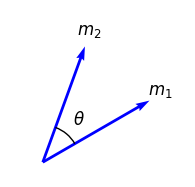
\includegraphics[scale=0.5]{angle_bound_example}
        \centering
        \caption{Picture of the bound of lemma 12.2}
        \label{fig:angle_bound_example}
    \end{figure}

    {\color{red} Are you going to use the results to improve the upper bound on the number of branch points in dimension $N \geq 3$. If so, then before stating the above lemma mention that it is tight, and that such a bound is not available in higher dimensions and that you will be using the next results to obtain such upper bounds.}


    \begin{theorem}
        \textbf{Angles bound \cite[Lemma 12.2]{Bernot}}
        Consider a vertex $s$ and two vertices $p_1, p_2$ connected to it. Let $m_1, m_2$ be the masses of the two edges leaving
        $s$ and connecting to $p_1, p_2$ respectively (see figure~\ref{fig:angle_bound_example}).
        Let $\theta$ be the angle between the two edges. Then, for every $\alpha \in [0,1]$:
        \begin{equation}
            \cos(\theta) \le \frac{(m_1 + m_2) ^ {2\alpha} - m_1^{2\alpha} - m_2^{2\alpha}}{2m_1^\alpha m_2^\alpha}
        \end{equation}
    \end{theorem}

    \begin{theorem}
        \label{lemma:bernot_angles_sum_bound}
        \textbf{Angles bound \cite[Lemma 12.5]{Bernot}}
        Consider a vertex $s$ and two terminals $s_1, s_2$ connected to it. Let $m_1, m_2$ be the masses of the two edges connecting
        $s$ to $s_1, s_2$ respectively. Let $\theta$ be the angle between the two edges.
        Then, for all $\alpha \in [0,1]$ and for all $m_1, m_2 \in [0,1]$:

        \begin{equation}
            \cos(\theta) \le \begin{cases}
                                 2^{2\alpha-1}-1 & \text{if} \frac{1}{2} < \alpha \le 1\\
                                 0 & \text{if 0} \le \alpha \le \frac{1}{2}\\
            \end{cases}
        \end{equation}

        Notice that this bound is independent of the masses of the edges. In the proof of the lemma it is also proved that the function
        \begin{equation}
            f(m_1) = \frac{(1+m_1)^{2\alpha} - 1 - m_1^{2\alpha}}{2m_1^\alpha}
        \end{equation}
        is decreasing for $m_1 \in [0,1]$ and $\alpha \in [0,\frac{1}{2}]$ and increasing for $m_1 \in [0,1]$ and $\alpha \in [\frac{1}{2},1]$.

        What about putting the above two lemmas in one statement as the second seems to be a simple consequence of the first one.

    \end{theorem}

    {\color{red} Again you need to motivate the following, otherwise, it seems completely irrelevant.}

    \begin{theorem}
        \textbf{Spherical cap results \cite[Theorem 1 and 2]{Rankin}}
        \label{definition:spherical_cap_results} \\
        The following result will be used to bound the number of branches in the optimal transport problem in~\ref{lemma:degree_definition}. \\
        Let $S_N$ denote the "surface" of an $N$-dimensional unit sphere in Euclidean space of
        $N$ dimensions. We may suppose that the sphere is centred at the origin of coordinates $O$
        By a spherical cap $Cap(\beta, N)$ of angular radius $\beta \le \pi$ and centre $P$ on $S_N$ , we mean the set of
        points $Q$ of $S_N$ for which the angle $QOP$ is less than or equal to $\beta$. Our object is to obtain an
        upper bound for the maximum number $C(\beta, N)$ of non-overlapping caps $Cap(\beta, N)$ which can be
        placed on $S_N$, and to investigate this upper bound for large values of $N$.
        \begin{enumerate}
            \item[(i)] \( C(\beta, N) = 1 \text{ for } \frac{1}{2}\pi < \beta \leq \pi; \)
            \item[(ii)] \( C(\beta, N) = \left\lfloor \frac{2 \sin^2 \beta}{2 \sin^2 \beta - 1} \right\rfloor \text{ for } \frac{1}{4}\pi + \frac{1}{2} \sin^{-1} \frac{1}{N} \leq \beta \leq \frac{1}{2}\pi; \)
            \item[(iii)] \( C(\beta, N) = N + 1 \text{ for } \frac{1}{4}\pi < \beta \leq \frac{1}{4}\pi + \frac{1}{2} \sin^{-1} \frac{1}{N}; \)
            \item[(iv)] \( C\left(\frac{1}{4}\pi\right) = 2N. \)
        \end{enumerate}

        If $0 < \beta < \frac{1}{4}\pi$ and $\gamma = \sin^{-1}\left(\frac{\sqrt{2} \sin \beta}{2}\right)$, then
        \begin{equation}
            C(\beta, N) \leq \frac{\pi \Gamma\left(\frac{N-1}{2}\right) \sin \gamma \tan \gamma}{2 \Gamma\left(\frac{N}{2}\right) \int_0^{\gamma} (\sin \phi)^{N-2} (\cos \phi - \cos \gamma) \, d\phi} = C^*(\beta)
        \end{equation}

        furthermore, for large $N$
        \begin{equation}
            C^*(\beta, N) \sim \frac{\frac{1}{2}\pi N^3 \cos 2\beta}{(\frac{\sqrt{2} \sin \beta}{2})^{N-1}}
        \end{equation}

        provided that $\sec 2\beta = o(N)$.
        \begin{figure}[h]
            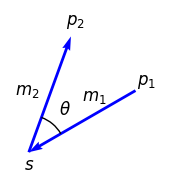
\includegraphics[scale=0.5]{angle_bound_example_inverted}
            \centering
            \caption{Picture of the bound of lemma 12.16}
            \label{fig:angle_bound_example_inverted}
        \end{figure}
    \end{theorem}


    \section{Main results}

    In this section, we present the main results, which provide lower bounds on the angles between edges.
    These bounds depend either on the specific instance of the problem $(\mu^{\pm}, N, \alpha)$ or only on the pair $(N, \alpha)$.
    Once we have these bounds, we can use the results for spherical cap packing~\ref{definition:spherical_cap_results}
    to obtain upper bounds on the number of branches in the optimal transport problem.

    The following lemma offers an improvement over~\cite[Lemma 12.16]{Bernot},
    where the competitor is considered along the edge instead of the span defined by the three vertices.

    \begin{lemma}
        \label{lemma:bound_opposite_direction}
        Consider a vertex $s$ and two terminals $s_1, s_2$ connected to it (as illustrated in \ref{fig:angle_bound_example_inverted}). Let $m_1, m_2$ be the masses of the two edges connecting
        $s$ to $s_1, s_2$ respectively, such that $m_1 \ge m_2$ and $m_1$ is flowing toward $s$ and $m_2$ is flowing away from $s$.
        Let $\theta$ be the angle between the two edges. Then, for every $\alpha \in (0,1]$:

        \begin{equation}
            \cos(\theta) \le \frac{(m_1 - m_2) ^ {2\alpha} - m_1^{2\alpha} - m_2^{2\alpha}}{2m_2^\alpha m_1^\alpha}
        \end{equation}

        \begin{proof}
            We can assume $p_1$ and $p_2$ lie on the unit circle by zooming enough and then rescaling, using the property that every restriction of an optimal
            solution is optimal~\cite[Chapter 8]{Bernot}. Calling the candidate new branching point $x$ and setting $s=(0,0)$.
            We can write the cost $f$ of this configuration of the tree as:
            \begin{equation}
                f(x) = m_1^{\alpha}\|p_1 - x \| + m_2^{\alpha} \|p_2 - x\| + (m_1-m_2)^{\alpha} \|x\|
            \end{equation}
            By setting $x = \epsilon v$ with $\|v\|=1$ and expanding to the first order around $\epsilon=0$:
            \begin{equation}
                f(\epsilon v) = f(0) - \epsilon m_1^{\alpha} v \cdot p_1 - \epsilon m_2^{\alpha} v \cdot p_2 + (m_1-m_2)^{\alpha} \epsilon + o(\epsilon)
            \end{equation}

            Given that we only want to check when $f(0)$ is not a maximum we can restrain our search around $\epsilon$ close to $0$.

            \begin{figure}[h]
                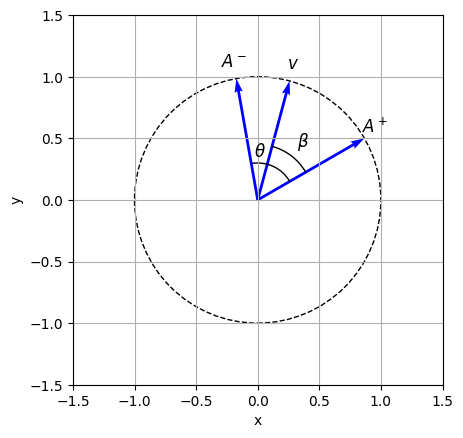
\includegraphics[scale=0.5]{circle}
                \centering
                \caption{Diagram of $p_1$, $p_2$ and $s$ for edges flowing in opposite directions}
            \end{figure}

            We can parametrize $v$ with the angle $\beta$ from $p_1$ (going toward $p_2$) and get to the following equation:
            \begin{equation}
                f(\epsilon) - f(0) = \epsilon \left[ (m_1-m_2)^\alpha - m_2^\alpha \cos\beta - m_1^\alpha (\cos\theta\cos\beta - \sin\theta\sin\beta) \right] + o(\epsilon)
            \end{equation}

            To prove that $\theta$ is not optimal we have two options:
            \begin{itemize}
                \item prove that there exists $\beta$ such that the first order coefficient is negative
                \item prove that the first order coefficient is bigger than $0$ for all $\beta$
            \end{itemize}


            To do this we want to fix $\theta, m_1, m_2$ and study the minimum of this function:
            \begin{equation}
            (m_1-m_2)
                ^\alpha - m_2^\alpha \cos\beta - m_1^\alpha (\cos\theta\cos\beta - \sin\theta\sin\beta)
            \end{equation}

            Calling $t = \cos(\beta)$ we get that the following equations needs to have a solution for $\beta$:
            \begin{equation}
                \label{eq:optimality_condition_proof}
                (m_1-m_2)
                ^{\alpha} + \cos\beta(-m_2^\alpha-m_1^\alpha t) + \sin\beta(m_1^\alpha \sqrt{1-t^2}) = 0
            \end{equation}

            Finding a value of $\beta$ such that this equation evaluates to 0 is not sufficient.
            We also need to verify whether this point corresponds to a local minimum.

            We know that there exists some $\beta$ for which this expression becomes negative (by choosing $\beta$ outside the
            span of $p_1$ and $p_2$, which contradicts the convex hull property of the optimal solution). Therefore, if $\theta$
            is not optimal, this function must cross zero.


            By solving equation \ref{eq:optimality_condition_proof}, using that $c^2 \le a^2 + b^2$ is a necessary and
            sufficient condition for an equation of the form $a\cos\beta + b\cos\beta = c$ to have a solution, we get:
            \begin{equation}
                \label{eq:optimality_condition_proof_2}
                t \ge \frac{(m_1-m_2)^{2\alpha} - m_1^{2\alpha} - m_2^{2\alpha}}{2m_2^\alpha m_1^\alpha}
            \end{equation}
        \end{proof}

    \end{lemma}
    We notice that~\ref{eq:optimality_condition_proof_2} is almost the same as~\cite[lemma 12.2]{Bernot}.
    In fact the only difference is that along the edge conencting $s$ to the branching point here we have the difference
    of the masses instead of the sum.

    \begin{lemma}
        \label{lemma:difference_bound_decreasing}
        The function:
        \begin{equation}
            f(m_1, m_2) = \frac{(m_1 - m_2) ^ {2\alpha} - m_1^{2\alpha} - m_2^{2\alpha}}{2m_2^\alpha m_1^\alpha}
        \end{equation}
        is decreasing in the ratio $\frac{m_2}{m_1}$ and that $\frac{m_2}{m_1} \rightarrow 0$ is $0$.

        \begin{proof}
            We notice $f$ is homogeneous and can therefore be reparametrized in terms of the ratio of the masses. Calling $m= \frac{m_2}{m_1}$
            we get:
            \begin{equation}
                f(m_1, m_2) = g(m_1/m_2) \coloneqq \frac{(1 - m) ^ {2\alpha} - 1 - m^{2\alpha}}{2m^\alpha}
            \end{equation}
            We can then verify that this function is indeed decreasing in $m$ as $(1-m)^ {2\alpha}$, $-m^{2\alpha}$
            and $1/ m^\alpha$ are all decreasing functions.
            Therefore
            \begin{equation}
                \sup_{m_1, m_2} f(m_1,m_2) = \lim_{m \rightarrow 0} g(m) = 0
            \end{equation}
            To compute the limit we apply de l'Hopital's rule and get:
            \begin{equation}
                \lim_{m \rightarrow 0} g(m) = \lim_{m \rightarrow 0} \frac{-2\alpha (1-m)^{2\alpha-1} - 2\alpha m^{2\alpha-1}}{2\alpha m^{\alpha-1}} = 0
            \end{equation}
        \end{proof}

    \end{lemma}

    \begin{lemma}
        \label{lemma:bound_general_direction}

        Let $\mathbf{P}$ be an optimal traffic plan transporting $\mu^+$ to $\mu^-$ with finite energy and finite graph structure.
        Consider a branching point $s$ located outside the support of $\mu^{\pm}$, with two branches connecting $s$ to points $x_1$ and $x_2$.
        Denoting the angle $\angle x_1 s x_2$ by $\theta$, the following inequality holds:

        \begin{equation}
            \label{eq:bound_general_direction}
            \cos(\theta) \le \max\left( 2^{2\alpha - 1} - 1, 0 \right).
        \end{equation}

        Furthermore, the degree is bounded by $C \left( \frac{\theta_{\max}}{2}, N \right)$, where $\theta_{\max}$
        is the angle that realizes the maximum in equation~\ref{eq:bound_general_direction}.

        \begin{proof}
            By combining lemmas~\ref{lemma:bound_opposite_direction} and~\ref{lemma:difference_bound_decreasing}, along with~\cite[Lemma 12.5]{Bernot}, we obtain a bound on $\cos \theta$ that applies to all masses and depends only on $\alpha$.

            Taking the supremum over all masses, we conclude that for a three-point system, there is no branching point if
            \begin{equation}
                \cos(\theta) \le \max \left( \max\left( 2^{2\alpha - 1} - 1, 0 \right), 0 \right).
            \end{equation}
        \end{proof}

    \end{lemma}

    \begin{corollary}
        In the case where $\mu^+$ and $\mu^-$ are two measures with finite support we know that lemma~\ref{lemma:bound_general_direction}
        holds also for points in their support.
    \end{corollary}

    \subsection{Discrete branched transport}

    The Discrete Branched Transport (DBT) is a special case of branched transport
    where the measures $\mu^+$ and $\mu^-$ are finite and atomic.

    Formally, we can define the DBT as follows: \\
    Given a dimension $N$, a cost parameter $\alpha$, and a set of terminal points $P = \{p_1, \ldots, p_n\}$ in $\mathbb{R}^N$ with
    corresponding masses $M = \{m_1, \ldots, m_n\}$, such that:
    \begin{itemize}
        \item $\sum_{i=1}^{n} m_i = 0$
        \item $P^+$ is the set of terminals with positive mass (sources) and $P^-$ is the set of terminals with negative mass (sinks)
    \end{itemize}

    the goal is to find a weighted graph $(S \cup P, E, f)$, where $S = \{s_1, \ldots, s_m\}$
    consists of Steiner points
        {\color{red} why are we calling these Steiner points? Is this terminology used in bracned transport? if yes, why didn't we use this name before?
    This terminology is used in the euclidean steiner tree problem and in the other formulation (MMX). Should I sttle for one and just say that they are synonim?
    }

    $s_i \in \R^N$, $E \subseteq S \cup P \times S \cup P$ is the set of edges and
    $f : E \rightarrow \mathbb{R}$ is the flow on each edge.
    The graph must form a network flow with sources ($P^-$) and sinks ($P^+$) at the terminal points in accordance with their masses,
    such that the following cost function is minimized:
    \[
        \sum_{(x,y) \in E} f_{xy}^\alpha \|x - y\|
    \]
        {\color{red} This notation is confusing; are $x,y$ nodes of the graph or the corresponding coordinates of terminals or Steiners?}
        {\color{red} What a negative flow means in your formulation. DONE}
    \begin{remark}
        It follows from~\ref{lemma:loop_free} that the optimal solution of a DBT problem is a union of trees.
        In the special case where there is only one source then the optimal solution is a tree becuase of the connectivity
        of the solution.
            {\color{red} why? this follows from Antonio's result, right? if so, cite it. DONE}
    \end{remark}
    \begin{remark}

        The problem remains unchanged if the signs of the masses are inverted, meaning that sources and sinks can be swapped.
        Therefore, it is sufficient to analyze either the case of a single source or a single sink, as they are the same problem.

            {\color{red} Why do we need this remark? Have you used this fact anywhere? Later we restrict to a single sink,
        it is just to say that the same applies also for a single source, but it is overall a very obvious fact}
    \end{remark}

    \subsection{Euclidean Steiner Tree problem}

    The ESTP is a special case of DBT, where  $\alpha=0$ and only a single source is present.
    This implies that the cost function is the sum of the lengths of the edges, and it does not take into account the flow on the edges.
    In this case, masses are irrelevant and the optimal solution is a tree connecting all the terminals.
    The objective function is then:
    \begin{equation}
        \sum_{(x,y) \in E} \|x - y\|
    \end{equation}
    {\color{red} Please fix the notation.}
    This special case has been extensively studied, especially computationally,
    and it is known that its decision version is NP-complete~\cite{karp2010reducibility}. {\color{red} fix?}

    \subsection{Instance specific bounds}

    We now have a bound on the cosine of the angle between two edges given their flows. In~\ref{lemma:bound_general_direction} we have
    taken the supremum over all possible masses to obtain an instance independent bound. {\color{red} Please specify the result you are referring to. DONE}
    We now focus on looking for a bound that holds at every branching point of a specific instance of the problem,
    so we assume that we already know the set $M$.

        {\color{red} You have a couple of results already depending on $m_1, m_2$. What you do mean we now focus on an instance specific bound?
    I think you mean you can find better bounds since you made additional assumptions on $\mu^-, \mu^+$, right? (as you describe below). If so, please revise this sentence. TODO: finisci}

    We now focus on the case where there is only one source and therefore the optimal solution is a tree.
    In this case, thanks to the loop-free property of the optimal solution, we know that the masses on the edges are
    combinations of masses in $M$. We can then maximize the bound of the cosine under this constraint to find the smallest
    angle that can be achieved in a specific instance of the problem.

    \begin{lemma}
        \label{lemma:degree_definition}
        Given an instance of a DBT problem with a single source ($p_0$), with masses $M=\{-1, m_1, \dots, m_n\}$
            {\color{red} why did you add $-1$ to the set of masses?}
        such that $\sum_{i =1}^{n} m_i = 1$, terminals $P=\{p_0, p_1, \dots, p_n\}$ and
        a cost parameter $\alpha \in (0,1)$, consider a branching point $s$ with two branches attached to it,
        calling the angle between them $\theta$ and defining $m_{\min} = \min_{i \in P^+} m_i$ we have:

        If $\alpha \le 1/2$:
        \begin{equation}
            \cos(\theta) \le \max\left(
            \frac{1 - m_{\min}^{2\alpha} - (1-m_{\min})^{2\alpha}}{2(m_{\min}(1-m_{\min}))^\alpha},
            \frac{(1-m_{\min})^{2\alpha} - m_{\min}^{2\alpha} - 1}{2m_{\min}^\alpha}
            \right)
        \end{equation}

        If $\alpha > 1/2$, define the ratio $r$ as:
        \begin{equation}
            \label{eq:ratio_definition}
            r = \max \left\{ \frac{m_i}{m_j} \text{  s.t.  } A_i, A_j \subseteq M, A_i \cap A_j = \emptyset, m_i = \sum_{k \in A_i} m_k, m_j = \sum_{k \in A_j} m_k, m_i \le m_j \right\}
        \end{equation}

        Then we have:
        \begin{equation}
            \cos(\theta) \le \max\left(
            \frac{ (1+r)^{2\alpha} - 1 - r^{2\alpha}}{2r^\alpha},
            \frac{(1-m_{\min})^{2\alpha} - m_{\min}^{2\alpha} - 1}{2m_{\min}^\alpha}
            \right)
        \end{equation}


        Defining $\theta_{\max}(M, \alpha)$ as the angle that achieves the maximum above, we can find an upper bound on the number of branches
        at any point of an optimal solution and define it as:
        \begin{equation}
            deg(M, N, \alpha) = C\left( \frac{ \theta_{\max}(M, \alpha) }{2}, N\right)
        \end{equation}

        Where $C$ is the function defined in~\ref{definition:spherical_cap_results}.
    \end{lemma}

    \begin{corollary}
        At a branching point outside of the support of $P$ we know that the conservation of flow holds, therefore there is
        at least one incoming edge and one outgoing edge. Given this we can slightly improve the bound with a strategy
        similar to~\cite[Section 11]{Bernot}.
            {\color{red} I dont understand. I am not sure that this is a useful remark/corollary}
    \end{corollary}
    \begin{remark}
        Finding $r$ as in~\ref{eq:ratio_definition} is probably computationally a difficult problem, so we could try some heuristic to find a good approximation.
        However, we need an upper bound on the ratio (rather than a lower bound) so it could be more difficult to obtain one (a feasible solution is
        not enough, we need a relaxation guarantee or a dual solution). We can empirically observe from
        (todo: include experiments from the notebooks) and~\ref{fig:first_bound_a_ge_1-2} that for most mass distributions there are subset with a ratio
        close to 1 and that we do not gain much by finding anything even with a $30\%$ error.
        So computationally it can make sense to just use $2^{2\alpha - 1} - 1$ as the bound.
    \end{remark}

    \begin{proof}
        We proceed in a similar way to~\ref{lemma:bound_general_direction}, but instead of taking the $\sup$
        over $m_1, m_2 \in [0,1]$ we maximize over the constraint that the masses on the branches $m_i,m_j$ are combinations of masses $M$.

        We have two bounds to consider: the first applies to the case where both edges flow outward,
        while the second applies to the case where one edge flows outward and the other flows inward.

        todo: first/second bound is an awful name

        \subsubsection{Optimizing the first bound}

        We aim to maximize:
        \begin{equation}
            f(m_i, m_j) = \frac{(m_i + m_j) ^ {2\alpha} - m_i^{2\alpha} - m_j^{2\alpha}}{2m_i^\alpha m_j^\alpha}
        \end{equation}

        Formally for the first bound, we know both edges are flowing out so the masses are "disjoint" (as a consequence of~\ref{lemma:loop_free}) in the sense that there
        exist sets $A_i, A_j \subseteq M$ such that $A_i, A_j \neq \emptyset$, $m_i = \sum_{k \in A_i} m_k$ and $m_j = \sum_{k \in A_j} m_k$ and $A_i \cap A_j = \emptyset$.

        Similarly to~\ref{lemma:difference_bound_decreasing} we can see that the function depends only on the ratio of the masses $m = \frac{m_i}{m_j}$. Rewriting it we get:

        \begin{equation}
            f(m) = \frac{(1 + m) ^ {2\alpha} - 1 - m^{2\alpha}}{2m^\alpha}
        \end{equation}

        We can also observe that $f(m) = f(1/m)$ so it is enough to consider $m \in [0,1]$.
        From~\ref{lemma:bernot_angles_sum_bound} we know that there is a different behaviour depending on $\alpha$ (figures \ref{fig:first_bound_a_le_1-2} and \ref{fig:first_bound_a_ge_1-2}).:
        \begin{itemize}
            \item If $\alpha \le 1/2$ we have that the function is decreasing in $m$. Therefore the maximum is achieved when $m$ is the smallest.
            \item If $\alpha > 1/2$ we have that the function is increasing in $m \in [0,1]$. The maximum is achieved when $m = 1$.
        \end{itemize}

        \subsubsection{Case $\alpha \le 1/2$}
        In the first case, it is sufficient to take
        \begin{align}
            & m_i = \min_{k \in M} |m_k| \\
            & m_j = \sum_{k \in M} m_k - m_i = 1 - m_i
        \end{align}

        \begin{figure}[h]
            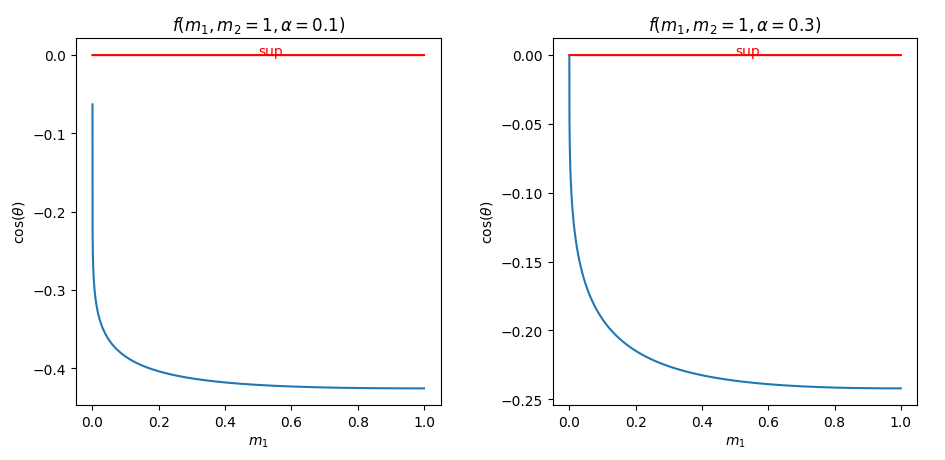
\includegraphics[scale=0.5]{f_sum_m1_m2_alpha_le_1-2}
            \centering
            \caption{Plot of the first bound for $\alpha \le 1/2$}
            \label{fig:first_bound_a_le_1-2}
        \end{figure}

        \subsubsection{Case $\alpha \ge 1/2$}

        The definition~\ref{eq:ratio_definition} is just a more compact way to write the solution to the optimization problem
        of finding the maximum ratio of two masses.

        \subsubsection{Optimizing the second bound}
        We are aiming at maximizing the function (see figure~\ref{fig:second_bound}):
        \begin{equation}
            f(m_i, m_j) = \frac{(m_i - m_j) ^ {2\alpha} - m_i^{2\alpha} - m_j^{2\alpha}}{2m_i^\alpha m_j^\alpha}
        \end{equation}
        We know from~\ref{lemma:difference_bound_decreasing} that this function only depends on $m = \frac{m_j}{m_i}$ and that the following:
        \begin{equation}
            f(m) = \frac{(1 - m)^{2\alpha} - m^{2\alpha} - 1}{2m^\alpha}
        \end{equation}
        is decreasing.

        We can now optimize the function over combinations of masses. Our objective is to minimize the ratio
        $m$. The two masses are independent so we conclude that the minimum is achieved when
        $m_i = \min_{k \in P^+} |m_k| \) and \( m_j = \sum_{k \in P^+} m_k = 1$.
    \end{proof}
    \begin{figure}[h]
        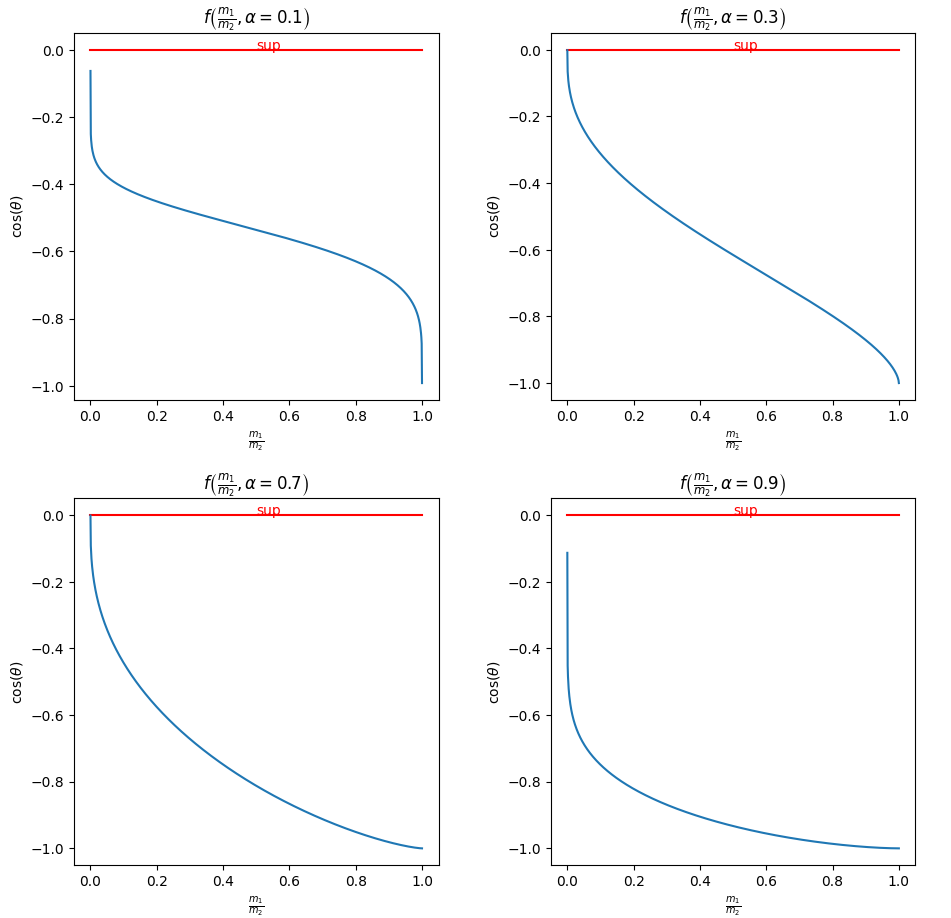
\includegraphics[scale=0.5]{f_diff_m1_m2}
        \centering
        \caption{Plot of the second bound}
        \label{fig:second_bound}
    \end{figure}



    \begin{figure}[h]
        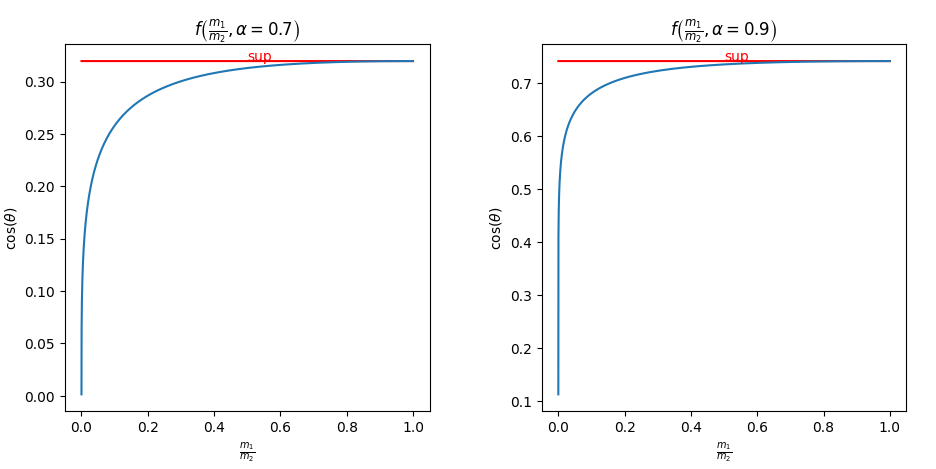
\includegraphics[scale=0.5]{f_sum_m1_m2_alpha_ge_1-2}
        \centering
        \caption{Plot of the first bound for $\alpha \ge 1/2$}
        \label{fig:first_bound_a_ge_1-2}
    \end{figure}


    \section{Minimum distance between branching points}

    In this section we aim to find a bound on the minimum distance between branching points. This result can then be added
    to the MINLP formulation to improve speed.

    \begin{lemma}
        Fix $\alpha \in (0,1)$ and $N$. For any $\delta > 0$ there exists $\mu^+ = \delta_{x_0}$ and $\mu^- = \sum_{i=1}^{4} m_i \delta_{x_i}$
        where $x_i \in \R^N$ and $m_i$ are the masses of the terminals such that in the optimal solution of the DBT problem the distance between
        the branching points smaller than $\delta$.
    \end{lemma}
    { \color{teal} I added this "lemma" to show that there is no good bound. There is a simple counterexample in
    the github repo in "converging\_steiner\_counterexample.py" }

    \begin{lemma}
        Fix $\alpha \in (0,1)$, $N$ and a compact subset $K \subseteq \R^N$. For any $\epsilon > 0$ there exists $\delta(\epsilon)$ such that for any $\mu^+ = \delta_{x_0}$ and $\mu^-$
        with support in $K$ and $\|\mu^-\| = 1$ we have that any optimal solution of the DBT has the following property:

        If two branching points $x_i, x_j$ are at $\epsilon$-distance from $supp(\mu^-)$ then the distance between them is at least $\delta(\epsilon)$.
    \end{lemma}

    \begin{proof}
        By contradiction, assume that there exists a $\epsilon > 0$ and a sequence of $\chi_n$ optimal solutions for $\mu^\pm_n$ such that
        there are two branching points for each $\chi_n$ called $x_i^n, x_j^n$ such that $\|x_i^n - x_j^n\| \rightarrow 0$ and $d(x_i^n, supp(\mu^-_n)) \ge \epsilon$.
        Up to passing to a subsequence we may assume that $x_i^n \rightarrow x$ and $x_j^n \rightarrow x$.

            {\color{teal}
        What to do now? Can I do a diagonalization argument to claim that I can do everything on finite graphs that converge to $\mu_+$?
        In that case what exactly is graph convergence? I assume converging as vector measures is equivalent to anything reasonable.
        }


    \end{proof}



    \section{Formulating DBT as a mathematical optimization problem}

    {\color{red} Put the general case first and then say in a remark by letting $\alpha = 0$ and the source to be a single Dirac delta, we obtain the Euclidean Steiner tree problem, and then give the formulation as well.}


    {\color{red} Get rid of MMX, give the optimization problems better names related to the problem name.}

    \subsection{DBT Formulation}

    In this section we present a formulation for the DBT problem with a cost parameter $\alpha$ and a
    single source $p^-=\{p_0\}$ based on~\cite[MMX]{mmx}.

    \begin{align}
        \text{(DBT)}: \; \min &\sum_{[i,j] \in E_1} f_{ij}^{\alpha}\|p_i - x^j\| + \sum_{[i,j] \in E_2} f_{ji}^{\alpha}\|x^i - x^j\| \\
        & \sum_{j \in S} y_{ij} = 1 \quad \text{for } i \in P \\
        & \sum_{k < j, k \in S} y_{kj} = 1 \quad \text{for } j \in S - \{p+1\}, \label{dbt_form:connectedness} \\
        & \sum_{i \in S} f_{ji} = m_j \quad \text{for } j \in P^+ \label{dbt_form:sum_terminals} \\
        & \sum_{i \in S} f_{ji} = -m_j \quad \text{for } j \in P^- \label{dbt_form:sum_sink} \text{todo: understand how to treat this in a decent way} \\
        & \sum_{i \in P} f_{ij} + \sum_{k < j, k \in S} f_{kj} + \sum_{k > j, k \in S} f_{jk} = 0 \quad \text{for } j \in S \label{dbt_form:sum_steiner_0}  \\
        & \sum_{i \in P} y_{ij} + \sum_{k < j, k \in S} y_{kj} + \sum_{k > j, k \in S} y_{jk} = 3 \quad \text{for } j \in S \label{dbt_form:degree_bound} \\
        & f_{ij} \le y_{ij} \quad \text{for } [i,j] \in E \\
        & s_i = \sum_{j \in P} c_{ij} p_j \\
        & y_{ij} \in \{0, 1\}, \quad [i, j] \in E, \quad x^i \in \mathbb{R}^n, \quad i \in S \\
        & f_{ij} \in [0,1] \quad \text{for } [i,j] \in E\\
        & c_{ij} \in \R_+ \quad i \in S, \quad j \in P
    \end{align}
    {\color{red} Also constrain $x^i$ to be in the convex hull of terminals DONE} \\
    {\color{red} Get rid of duplicates like $y_{ij}$ and $y_{ji}$. DONE} \\
    {\color{red} why $f_{ij}$ and $y_{ij}$ are defined over different index sets? The index set over which $f_{ij}$ as defined does not seem correct. It should either be between two Steiners $i,j$ or a Steiner $i$  and a terminal $j$ (similar to what you did in MMX for Steiner). DONE} \\
    where we define the followings:

    \begin{itemizeb}
        \leftskip 0.8 cm\labelsep=.3 cm
        \item [$P$] is the set of terminals $\{p_1, \ldots, p_n\}$,
        \item [$S$] is the set of Steiner $\{s_1, \ldots\}$ points (indexed as $S = \{|P| + 1, \dots, 2|P|-2\}$),
        \item [$E_1$] is the set of edges connecting terminals to Steiner points, such that $(i,j) \in E_1$ when $i \in P$ and $j \in S$.,
        \item [$E_2$] is the set of edges connecting Steiner points, such that $(i,j) \in E_2$ if $i,j \in S$ and $i < j$.
    \end{itemizeb}

    \begin{itemizeb}
        \leftskip 0.8 cm\labelsep=.3 cm
        \item[$\alpha \in (0,1)$] is the cost parameter
        \item [$M$] is the set of masses $\{m_1, \ldots, m_n\}$ of the terminals
        \item [$f_{ij}$] flow on the oriented edge $(i, j) \in E$  {\color{red} inconsistent notation.}
        \item [$y_{ij}$] binary variable indicating the presence of an un-oriented edge connecting $i$ to $j$  {\color{red} inconsistent notation.}
        \item [$ deg(\alpha, N, M)$] maximum degree of a vertex in the graph as defined in~\ref{lemma:degree_definition}
    \end{itemizeb}

    \subsection{Proof of correctness}

    When we say correctness we mean that, given an optimal solution of the DBT formulation we can reconstruct one of the optimal solutions
    to the DBT problem.
    Therefore we need to construct a function $\phi$ that maps feasible solutions of the formulation into feasible solutions of DBT (which are graphs)
    and prove that the optimality is preserved.

    Outline of the proof:
    \begin{enumerate}
        \item construction of the map that takes feasible solutions to graphs
        \item proof that flows are correct {\color{teal} write this properly}
        \item proof that the objective functions are the same
        \item proof of optimality for connected optimal solution where terminals are leaves and branching points have degree 3
        \item proof of optimality for connected optimal solution where terminals are leaves {\color{teal} TODO: this is what we need to correct}
        \item proof of optimality for connected optimal solution
    \end{enumerate}

    \subsection{Step 1}
    We define a function $\phi$ that maps $\mathbb{R}^{N (|P|-2)} \times \{0,1\}^{|E|} \times \R^{|E|}$ to a oriented weighted graph in $\mathbb{R}^N$ as follows:

    \begin{enumerate}
        \item For each $i \in P$, add a terminal at $p_i$.
        \item For each $j \in S$, add a vertex $s_j \in \R^N$ with coordinates $x^j$.
        \item If there are multiple vertices with the same coordinates, collapse them into one and identify them with any of the indices.
        \item For each $[i,j] \in E$ with $y_{ij} = 1$, add an edge between $v_i$ and $v_j$.
        \item Assign the flow $f_{ij}$ to the edge connecting $v_i$ to $v_j$. Note that either $(i,j) \in E$ or $(j,i) \in E$ but not both so flows
        cannot cancel.
    \end{enumerate}

    Note that this function is not injective, as we can permute the indices of the Steiner points and still get the same graph.
    We first show that $\phi(GMMX)$ is a feasible solution of DBT. Clearly, it is a graph so we are left to prove that the flow
    constraints work.

    The (only) source is a special terminal, and here we constraint it to be connected to $x_{|P|+1}$, the first Steiner point~\ref{dbt_form:sum_sink}.

    We observe that the constraints form a tree were leaves are sink terminals, so in any optimal solutions the flows all go "downstream".
    For any terminal $p$, in $\phi(GMMX)$ we could have a (possibly empty) set of degenerate steiner points, called $S_p = \{s_1, \dots, s_m\}$,
    at the same coordinates.
    The total flow of the collapsed vertex is:
        {\color{teal} FINISCI QUI CON CARTA E PENNA}
    \begin{equation}
        \sum_{i \in S} f_{ip} = m_p
    \end{equation}
    By constraint~\ref{dbt_form:sum_steiner_0} and~\ref{dbt_form:sum_terminals} we get that the final flow is exactly $m_p$.

    We can apply the same construction also for coinciding Steiner points. {\color{teal} FINISCI ANCHE QUI}

    Outside of any terminal the same computations yield a sum of $0$.
    We have also proved now that the set of feasible solutions of GMMX is a subset of the set of feasible solutions of DBT through $\phi$.
    This means that to prove the equivalence we only need to show that for any optimal solution in DBT
    there is a corresponding optimal solution in GMMX that maps to it.

    \subsection{Step 2}
    By calling $GMMX$ and $DBT$ the feasible regions of the respective problems, we show that the following diagram commutes:
    \[
        \begin{tikzcd}
            & \mathbb{R}  \\
            GMMX \arrow[ur, "Obj"] \arrow[rr, "\phi"'] & & DBT  \arrow[ul, "Obj"]
        \end{tikzcd}
    \]

    The objective function in GMMX is the sum of $(f_{ij} + f_{ji})^\alpha$ which is, after passing through $\phi$, the flow
    along the edge $(i,j)$, weighted by $\| p_i - x^j \|$ or $\|x^i-x^j \|$ which are the euclidean distances between
    Steiner points and terminals.
    The fact that there could be a degeneracy is not important as those points have $0$ distance and do not contribute to the
    objective value.

    \subsection{Step 3}

    We now show that there is an element in $GMMX$ that maps to a connected optimal solution of DBT where terminals are leaves.
    For each steiner point $s_i$ in the graph we can set $x^i = s_i$. We then set $y_{ij} = 1$ and $f_{ij}, f_{ji}$ to
    the appropriate value for each edge $(i,j)$ in the optimal solution of DBT. We are not violating the degree constraints
    as we are mapping an optimal solution of DBT.
    By an edge counting argument (crucially using that the solution is a tree) we can show that there are enough Steiner points to connect all the terminals.
    \begin{equation}
        |S| + |P| - 1 = \frac{1}{2} \left( 3|S| + \sum_{i \in P} d(i) \right)
    \end{equation}
    Which implies that:
    \begin{equation}
        \label{eq:edge_counting}
        \sum_{i \in P} d(i) = 2|P| - 2 - |S|
    \end{equation}

    because in our case $d(i)=1$ by assumption.
    In order to satisfy the connectivity constraint~\ref{dbt_form:connectedness} we have to re-order
    the steiner points in a topological order, which exists as it is a tree.

    \subsection{Step 4}
    Now we tackle the case where the terminals can have degree higher than $1$. We will show that we can add more degenerate
    steiner points to the graph until we reduce it to the case where all terminals are leaves. During this procedure we
    need to track how many steiner points we add.
    From equation~\ref{eq:edge_counting} we know that for every "extra" degree we have one extra Steiner point to work with.
    Define the following procedure:
    \begin{enumerate}
        \item Consider a terminal $p_i$ with degree $d(i)$ connected to points $\{x_1, \dots, x_{d(i)}\}$
        \item Add $d(i) - 1$ degenerate steiner points $\{s_1, \dots, s_{d(i)-1}\}$ at the same coordinates as $p_i$
        \item Connect them with edges $\{ (p_i, s_1), (s_1, s_2), \dots, (s_{d(i)-1}, x_{d(i)}) \}$
        \item Connect also edges $\{ (s_i, x_i) \}$ for $i = 1, \dots, d(i)-1$
    \end{enumerate}
    This procedure preserves the connectedness of the graph and its topology. We can repeat this procedure until all terminals
    have degree $1$.
    Once the topology is fixed, the flows are uniquely determined by the masses on the terminals. We might just have to
    re-order the Steiner points to satisfy the connectivity constraint~\ref{dbt_form:connectedness}.

    \subsection{Step 5}
    In the case of a disconnected optimal solution we would have a finite union of $T$ trees, where each tree is an optimal solution
    to a subproblem of the DBT. We can find a solution in GMMX of each tree using only $|P| - T$ Steiner points.
    We can use the remaining $T-1$ steiner points to connect the trees, by adding a Steiner point on an arbitrary terminal
    of each tree and connecting them with an edge of flow $0$. We then have to re-order steiner points to satisfy the connectivity.


    \begin{remark}
        The case of disjoint trees can only occur if there are multiple sources. In this case there is a symmetry in the ordering
        of the trees and this can heavily slow down solvers.
    \end{remark}

    \subsection{MMX}
    This formulation is due to~\cite[Section 2]{mmx}
    \begin{align}
        \text{(MMX)}: \; \min &\sum_{[i,j] \in E_1} \|p_i - s_j\| y_{ij} + \sum_{[i,j] \in E_2} \|s_i - s_j\| y_{ij}, \\
        & \sum_{j \in S} y_{ij} = 1 \quad \text{for } i \in P^+, \\
        & \sum_{i \in P} y_{ij} + \sum_{k < j, k \in S} y_{kj} + \sum_{k > j, k \in S} y_{jk} = 3 \quad \text{for } j \in S, \label{MMX:connectivity_steiner} \\
        & \sum_{k < j, k \in S} y_{kj} = 1 \quad \text{for } j \in S - \{p+1\},  \\
        & s_i = \sum_{j \in P} c_{ij} p_j \\
        & y_{ij} \in \{0, 1\}, \quad [i, j] \in E, \quad s^i \in \mathbb{R}^n, \quad i \in S \\
        & c_{ij} \in \R_+ \quad i \in S, \quad j \in P,
    \end{align}

    Where:
    \begin{itemizeb}
        \leftskip 0.8 cm\labelsep=.3 cm
        \item [$P$] is the set of terminals $\{p_1, \ldots, p_n\}$,
        \item [$S$] is the set of Steiner $\{s_1, \ldots\}$ points (indexed as $S = \{|P| + 1, \dots, 2|P|-2\}$),
        \item [$E_1$] is the set of edges connecting terminals to Steiner points, such that $(i,j) \in E_1$ when $i \in P$ and $j \in S$.,
        \item [$E_2$] is the set of edges connecting Steiner points, such that $(i,j) \in E_2$ if $i,j \in S$ and $i < j$.
    \end{itemizeb}

    We will prove its correctness by showing that the generalization of this formulation is equivalent to the DBT problem.


    \section{Numerical results}

    \newpage
    \printbibliography


\end{document}